\documentclass[10pt,letterpaper,twocolumn]{article}
\usepackage[margin=0.75in]{geometry}
\usepackage{graphicx}
\usepackage{float}
\usepackage{microtype}
\usepackage{titlesec}
\usepackage{caption}
\usepackage{parskip}
\setlength{\parskip}{0.25em}
\setlength{\parindent}{0pt}
\captionsetup{font=small}
\titleformat\section{\large\bfseries}{\thesection}{0.6em}{}
\titleformat\subsection{\normalsize\bfseries}{\thesubsection}{0.5em}{}

\begin{document}

\begin{center}
{\LARGE \textbf{Media vs. Public Opinion on GLP-1 Weight Loss Drugs}}\\
\vspace{0.3em}
INSY 669 - Text Analytics | McGill University | Winter 2026\\
\vspace{0.6em}
Vasilis Christopoulos (261278396) \hfill Hugo Guideau (261261108)\\
Saksi Khosla (261284778) \hfill Othmane Zizi (261255341)\\
Mustafa Yousuf (261265412)
\end{center}

\section{Introduction}
GLP-1 receptor agonists such as Ozempic (semaglutide) and Wegovy are discussed simultaneously in patient communities and in mainstream media. Those two discourse spaces can shape different expectations about safety, efficacy, cost, and access. This study quantifies where those narratives align and where they diverge using a fully refreshed run of the project pipeline on the fixed 2024 collection window.

The corpus contains 1,286 public documents (1,184 Reddit posts and 102 WebMD reviews) and 647 media documents (647 news items). The analytical goal is to compare the two corpora along six dimensions: sentiment, lexical overlap, classifier separability, topic structure, aspect-level framing, and temporal coupling.

\begin{table}[H]
\centering
\caption{Run quality and representation checks (hybrid snapshot).}
\begin{tabular}{l r}
\hline
Metric & Value \\
\hline
Public documents & 1,286 \\
Media documents & 647 \\
Body coverage & 0.696 \\
Fallback ratio & 0.304 \\
Reddit / WebMD / News & 1,184 / 102 / 647 \\
\hline
\end{tabular}
\end{table}

\section{Methodology}
\textbf{Collection strategy and data types.} Public data were collected from Reddit (community posts) and WebMD (patient reviews), while media data were collected from Google News RSS using GLP-1 specific query terms and then expanded with article-body extraction. This yields mixed data types: short conversational posts, semi-structured patient reviews, and long-form news articles.

\textbf{Hybrid representation rationale.} Media text was processed with \texttt{media\_text\_mode=hybrid}, which prefers extracted article body text and falls back to RSS snippet text only when body text is unavailable. This representation is appropriate for balancing semantic richness and coverage across heterogeneous publishers. In the frozen run, usable body coverage is 0.696 and fallback ratio is 0.304 (197/647).

\textbf{Information retrieval and preprocessing.} Retrieval combines API-style subreddit extraction, website scraping, RSS search aggregation, URL resolution, and HTML text extraction. Text preprocessing includes tokenization, lowercasing, punctuation and stopword filtering, and lemmatization. TF-IDF and Bag-of-Words feature spaces support comparison, classification, and clustering tasks.

\textbf{Experimentation process.} The pipeline was run sequentially with completion checks rather than partial assumptions. A strict first attempt used body timeout 15 and minimum body tokens 80. Because body coverage was insufficient, a second attempt used timeout 25 and minimum body tokens 60. The second attempt satisfied all representation gates and became the reporting snapshot.

\textbf{Hyperparameter tuning.} Classification used leakage-safe, cross-validated pipelines. Multinomial Naive Bayes tuned smoothing ($\alpha$) and KNN tuned neighborhood size ($k$) inside cross-validation. A robustness track repeated lexical and classification comparisons under token-length normalization (cap = 40 tokens) to test sensitivity to document length effects.

\section{Results}
\subsection{Sentiment Analysis}
Public and media sentiment distributions differ significantly. Mean VADER polarity is 0.1117 for public discourse and 0.1905 for media discourse (t = -2.301, p = 0.021516, Cohen's d = -0.108). The effect size is small, but statistically detectable at corpus scale.

Interpretively, public content remains more mixed because personal journey narratives include both benefit reports and adverse-experience accounts, whereas media language is more likely to be templated around explanatory health reporting and policy narratives.

\begin{figure}[t]
\centering
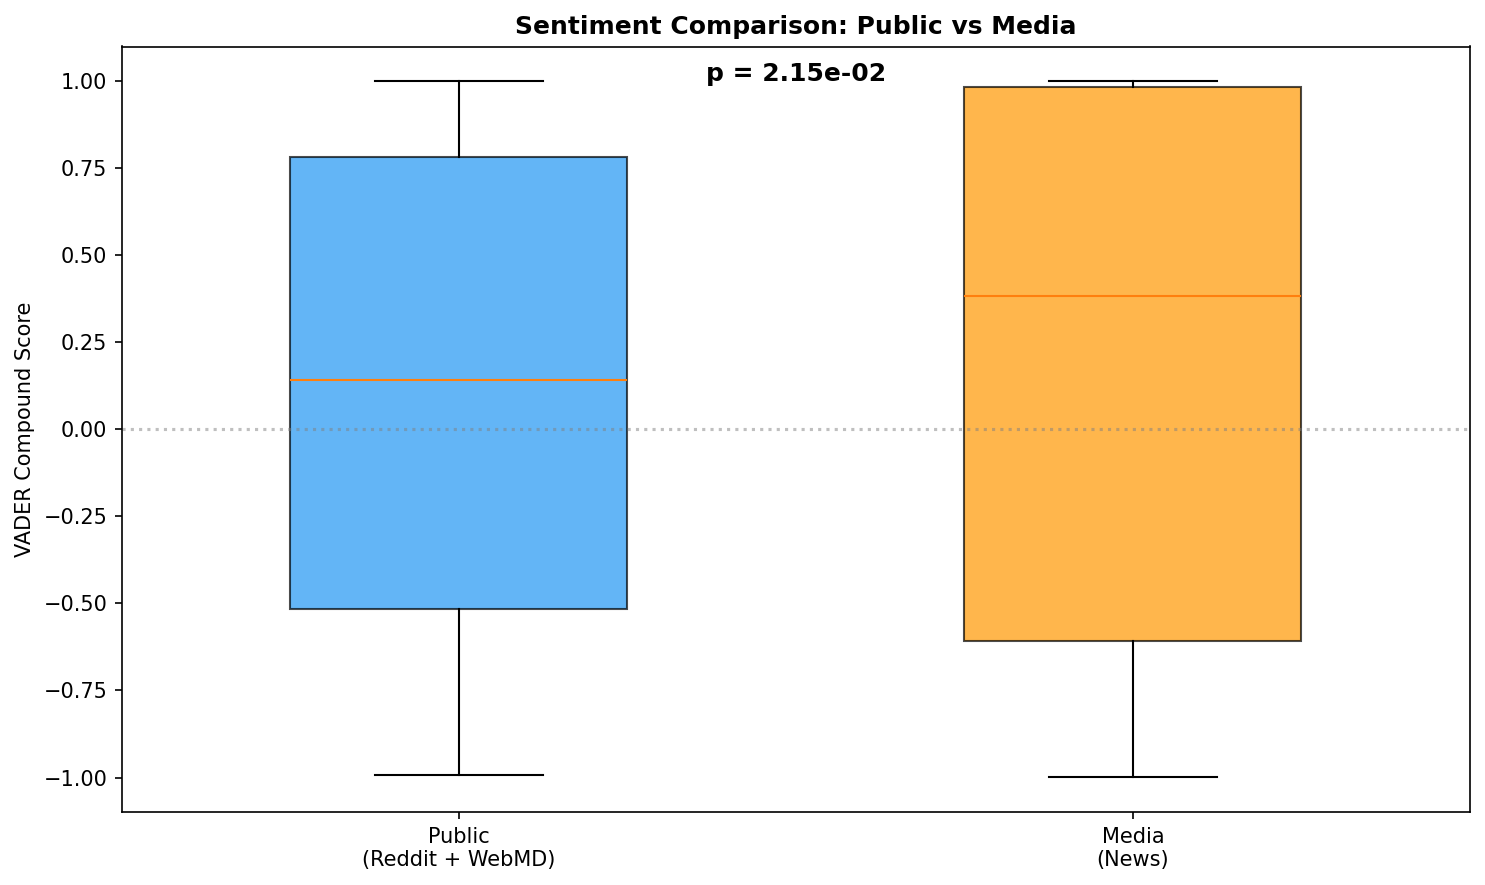
\includegraphics[width=0.95\columnwidth]{../figures/sentiment_boxplot.png}
\caption{Sentiment comparison between public and media corpora (hybrid mode).}
\end{figure}

\subsection{Corpus Comparison}
Lexical similarity is moderate at corpus level (cosine similarity = 0.446), and remains moderate under normalization (Norm40 cosine = 0.370). This pattern indicates shared topic anchors (drug names, efficacy, side effects) but distinct phrasing and contextual framing.

Side-effect framing differs materially in emphasis. For example, nausea prevalence in public documents is 0.0778 versus 0.0093 in media documents, showing that symptom reporting is more common in patient-authored text.

\begin{figure}[t]
\centering
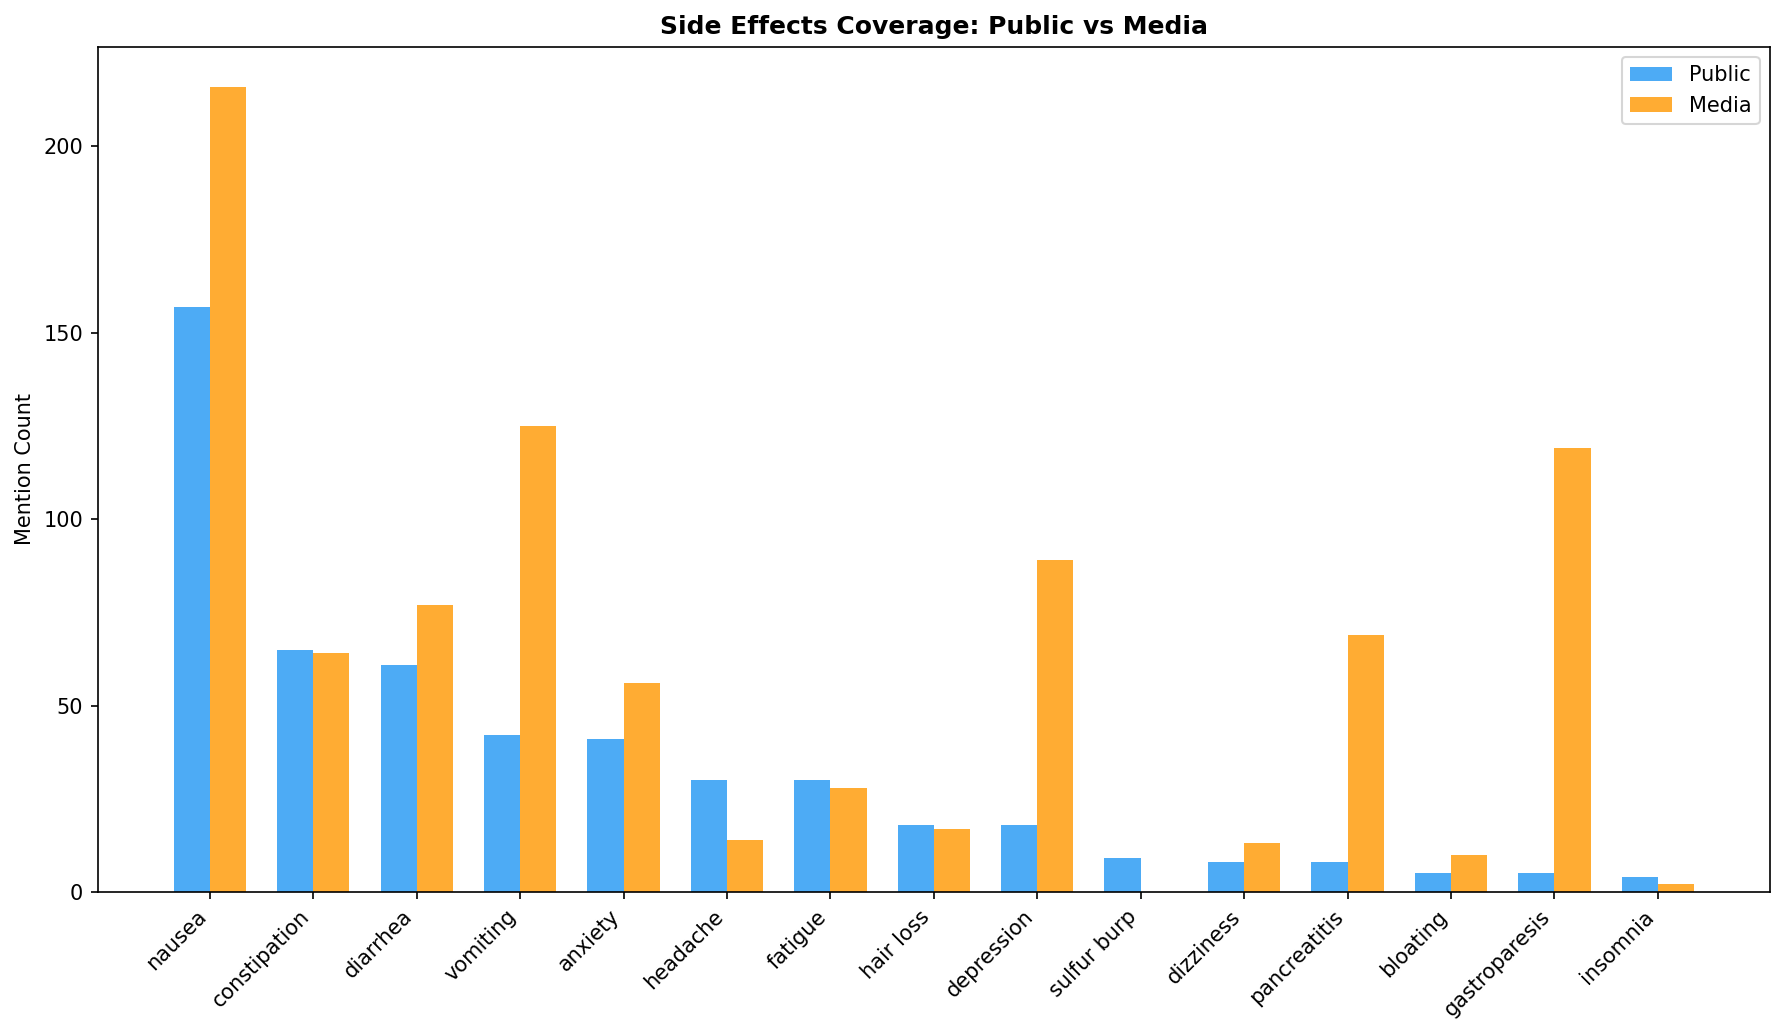
\includegraphics[width=0.95\columnwidth]{../figures/side_effects.png}
\caption{Side-effect mention counts in public versus media corpora.}
\end{figure}

\subsection{Text Classification}
The two corpora are strongly separable in supervised classification. In leakage-safe 5-fold CV, Multinomial Naive Bayes reaches 0.9783 accuracy (best $\alpha$ = 0.1) and KNN reaches 0.9550 (best $k$ = 5). Under normalization, Naive Bayes remains 0.9757 and KNN improves to 0.9710, confirming that separability is not only a by-product of length differences.

These results indicate robust discourse-style divergence: public language is experiential and first-person, while media language is institutional, attribution-heavy, and policy-oriented.

\begin{figure}[t]
\centering
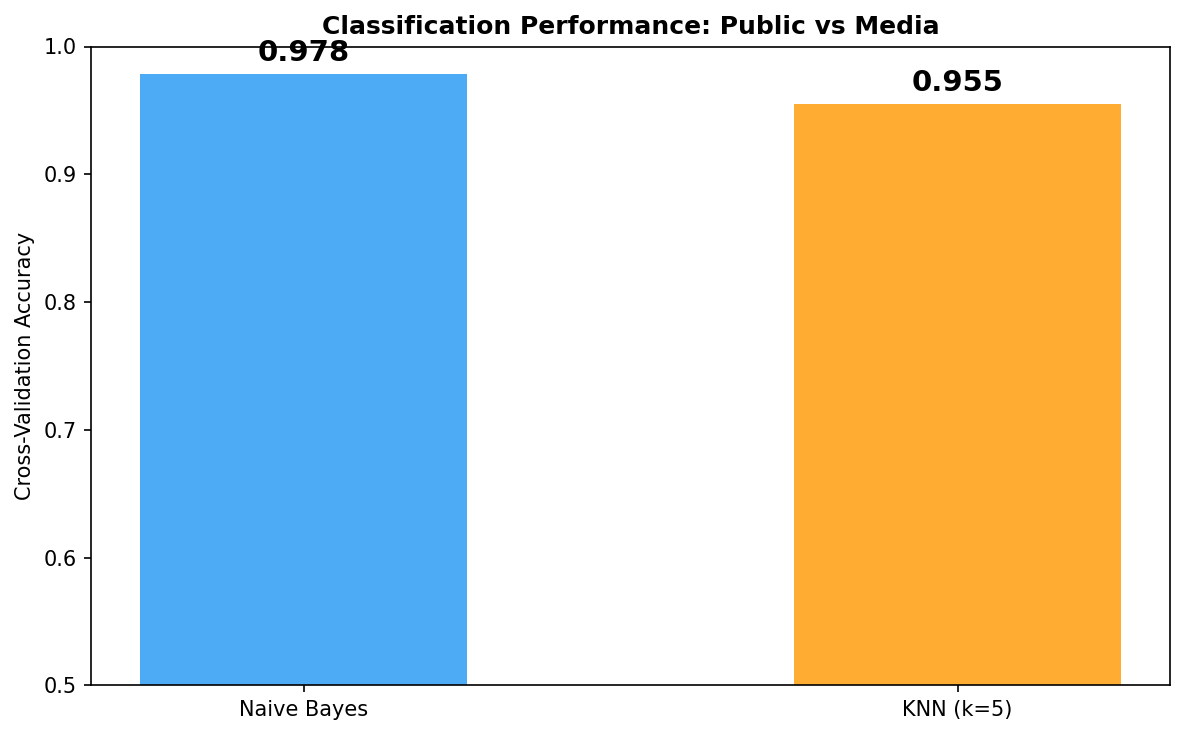
\includegraphics[width=0.95\columnwidth]{../figures/classification_comparison.png}
\caption{Cross-validated classification performance (NB vs KNN).}
\end{figure}

\subsection{Topic Modeling}
Topic modeling shows consistent thematic separation. Public topics are dominated by dosage progression, weight-change tracking, and day-to-day side-effect management. Media topics center on approvals, clinical evidence, shortages, and insurance-access framing. K-Means purity (0.898) supports this structural separation.

\subsection{Aspect-Based Sentiment}
Aspect-level sentiment reveals where framing differs most. Discrepancy scores (public minus media) are strongest for cost (-0.187), access (-0.132), and side effects (-0.174). Public discourse tends to encode these topics through direct personal experience, while media language is comparatively explanatory and policy-framed.

\subsection{Temporal Analysis}
Temporal coupling is weak. Cross-correlation peaks at lag -4 weeks (r = -0.2763), weekly volume correlation is 0.1894, and Granger tests are not significant in either direction (media->public p = 0.76723, public->media p = 0.518258). The two streams appear contemporaneously related but not strongly directional in this window.

\section{Discussion}
Three findings are stable in this refreshed hybrid run. First, discourse spaces remain clearly separable by language features, even after normalization-based robustness checks. Second, side-effect and access/cost framing are not symmetric across sources, with public posts carrying more direct adverse-experience emphasis. Third, weak temporal directionality suggests that weekly discourse changes are likely co-evolving rather than consistently led by one source.

A practical limitation is source heterogeneity: Reddit posts are shorter and conversational, WebMD reviews are structured but smaller in count, and news content varies by publisher formatting. Hybrid mode mitigates this by preferring full bodies while preserving coverage through controlled snippet fallback.

\newpage
\section{Conclusion}
Using recollected data and hybrid media representation, this analysis confirms persistent narrative divergence between public discourse and media framing on GLP-1 drugs. The conclusions are grounded in explicit representation quality gates, reproducible end-to-end execution, and leakage-safe modeling, and they remain directionally consistent across multiple analytical methods.

\vfill
\begin{center}
\small Snapshot run ID: 20260218\_185202\_hybrid\_recollect
\end{center}

\end{document}
